\documentclass{standalone}
% \documentclass{article}
\usepackage[T1]{fontenc}
\usepackage[utf8]{inputenc}
\usepackage{lmodern}
\usepackage{tikz}
\usetikzlibrary{arrows,calc}
\begin{document}
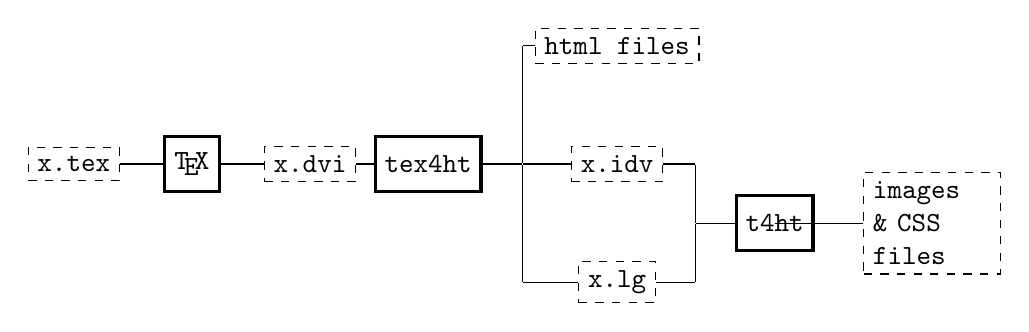
\begin{tikzpicture}[node distance=15mm, empty/.style={inner sep=0,minimum size=0},file/.style={rectangle,dashed,draw=black}, command/.style={rectangle,minimum size=2em,very thick,draw=black},font=\ttfamily,draw=black]
  \node (xtex) [file] {x.tex};
  \node (TeX) [command,right of=xtex] {\TeX};
  \node (xdvi) [file,right of=TeX] { x.dvi };
  \node (tex4ht) [command,right of=xdvi] {tex4ht};
  \node (split) [empty,right of=tex4ht,node distance=12mm] {};
  \node (split above) [empty, above of=split] {};
  \node (split below) [empty, below of=split] {};
  \node (xidv) [file,right of=split,node distance=12mm] {x.idv};
  \node (html) [file,above of=xidv] {html files};
  \node (xlg) [file,below of=xidv] {x.lg};
  \node (split right) [empty,right of=xidv,node distance=10mm] {};
  \node (split right down) [empty,right of=xlg,node distance=10mm] {};
  \node (join) [empty] at ($(split right)!0.5!(split right down)$) {};
  \node (t4ht) [command,right of=join,node distance=10mm] {t4ht};
  \node (pictures) [file,right of=t4ht,node distance=20mm,text width=15mm] {images \& CSS files};
  \draw  (xtex) to (TeX) to (xdvi) to (tex4ht) to (split) to (xidv);
  \draw  (split) -> (split above) -> (html);
  \draw  (split) -> (split below) -> (xlg);
  \draw (xidv) -> (split right) -> (join);
  \draw  (xlg) -> (split right down) -> (join)  -- (t4ht) |- (pictures);
\end{tikzpicture}

\end{document}
